\documentclass[tikz]{standalone}
\usetikzlibrary{arrows,shapes,matrix}

\begin{document}
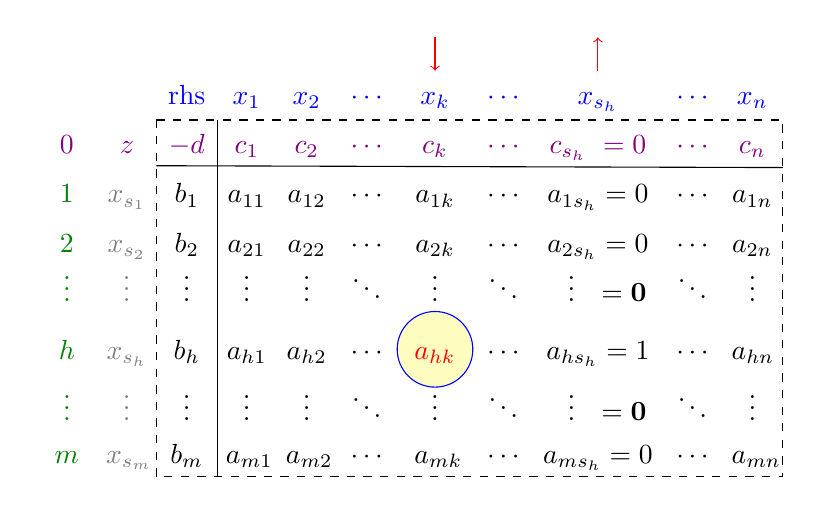
\begin{tikzpicture}
\node[row 1/.style=red,row 2/.style=blue, row 3/.style=red!50!blue,column 1/.style=green!50!black,column 2/.style=gray,cell/.style=rectangle,text height=2ex,text width=1.5em, align=center,column 9/.style={text width=4em},matrix of math nodes,scale=0.5] (tableau)
{
&&&&&&\draw[->] (0,12pt) -- (0,0pt);&&\draw[->] (0,0) -- (0,12pt);\\
&  &  \mbox{rhs}&  x_1 &  x_2 &  \cdots &  x_k &  \cdots &  x_{s_h} &  \cdots &  x_n\\
0& z &  -d &  c_1 &  c_2 &  \cdots &  c_k &  \cdots &  c_{s_h}~=0&  \cdots &  c_n\\
1& x_{s_1} &  b_1 &  a_{11} &  a_{12} &  \cdots &  a_{1k} &  \cdots &  a_{1{s_h}}=0 &  \cdots &  a_{1n}\\
2& x_{s_2} &  b_2 &  a_{21} &  a_{22} &  \cdots &  a_{2k} &  \cdots &  a_{2{s_h}}=0  &  \cdots &  a_{2n}\\
\vdots & \vdots &  \vdots &  \vdots &  \vdots &  \ddots &  \vdots &  \ddots &  ~~\vdots~~=\mathbf{0}  &  \ddots &  \vdots\\
h& x_{s_h} &  b_h &  a_{h1} &  a_{h2} &  \cdots &  \node[red, draw=blue, shape=circle,fill=yellow!25,opacity=1] {a_{hk}}; &  \cdots &  a_{h{s_h}}=1 &  \cdots &  a_{hn}\\
\vdots& \vdots &  \vdots &  \vdots &  \vdots &  \ddots &  \vdots &  \ddots &  ~~\vdots~~=\mathbf{0} &  \ddots &  \vdots\\
m& x_{s_m} &  b_m &  a_{m1} &  a_{m2} &  \cdots &  a_{mk} &  \cdots &  a_{m{s_h}}=0&  \cdots &  a_{mn}\\
};
\draw[sloped=0] (tableau-3-3.south west) -- (tableau-3-11.south east);
\draw[sloped=0] (tableau-3-3.north east) -- (tableau-9-3.south east);
\draw[dashed] (tableau-3-3.north west) -- (tableau-3-11.north east) -- (tableau-9-11.south east) -- (tableau-9-3.south west) -- cycle;
\end{tikzpicture}%
\end{document}
